% Goal: Draft of a revised Figure 1 for the conceptual framework paper, organized around the decision
% Andie Creel / Started November 2026
%
% DRAFT for discussion. Not yet in concept_frame_manuscript/draft_concept_framework.tex.
% Top row: how nature produces value (what existing frameworks explain).
% Bottom half: what this framework adds (many decision-makers, the slice each one sees, valuation closing the loop).

\documentclass[12pt]{article}
\usepackage[english]{babel}
\usepackage[letterpaper,landscape,top=1.5cm,bottom=1.5cm,left=2cm,right=2cm]{geometry}
\usepackage{graphicx}
\usepackage{tikz}
\usetikzlibrary{arrows.meta, decorations.pathreplacing, positioning, fit, backgrounds}
\pagestyle{empty}

\begin{document}
\centering
\resizebox{0.85\textwidth}{!}{%
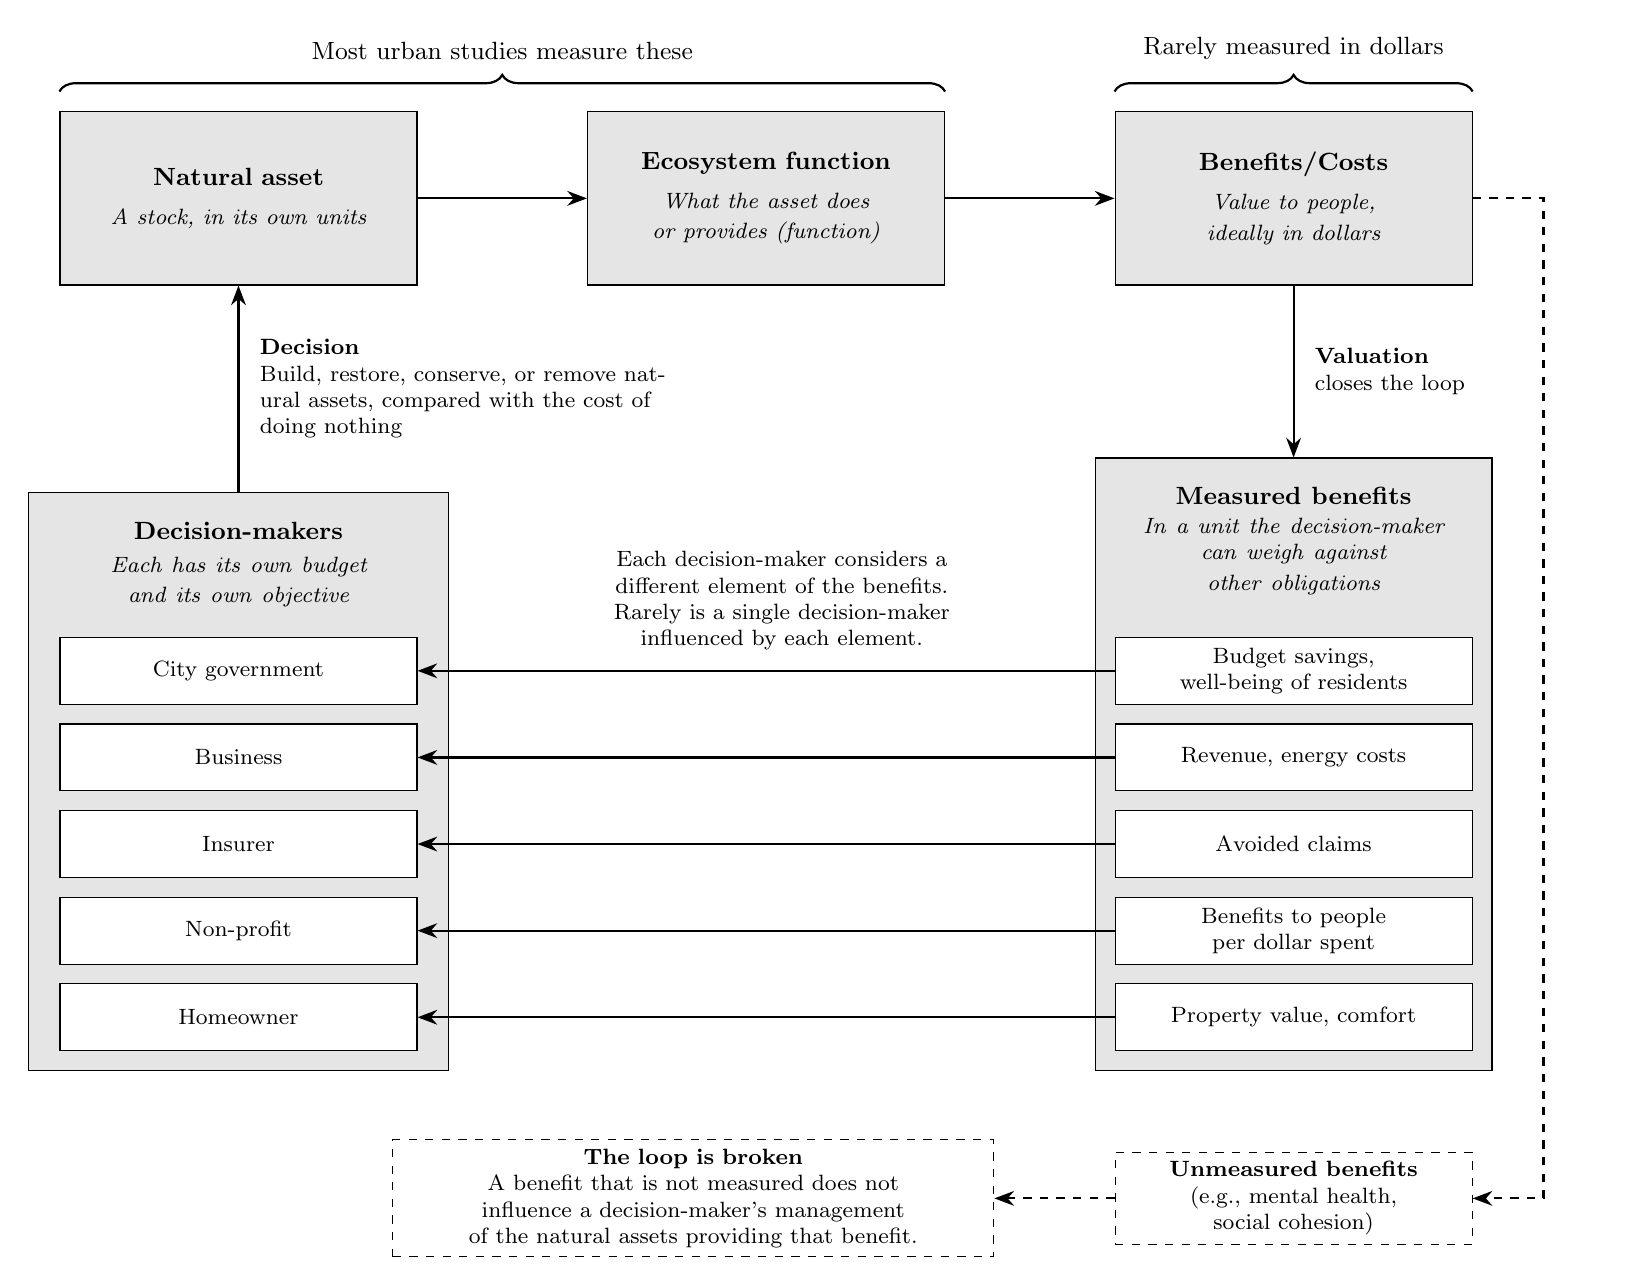
\begin{tikzpicture}[
  font=\small,
  head/.style={draw, fill=gray!20, text width=4.3cm, minimum height=2.2cm, align=center},
  small/.style={draw, fill=white, text width=4.3cm, minimum height=0.85cm, align=center, font=\footnotesize},
  grp/.style={draw, fill=gray!20, inner sep=7pt},
  arr/.style={-{Stealth[length=2.5mm]}, thick},
  lab/.style={align=center, font=\footnotesize}
]
  % ---------------- Top row: how nature produces value ----------------
  \node[head] (a) at (0,0)    {\textbf{Natural asset}\\[3pt]{\footnotesize\itshape A stock, in its own units}};
  \node[head] (s) at (6.7,0)  {\textbf{Ecosystem function}\\[3pt]{\footnotesize\itshape What the asset does or provides (function)}};
  \node[head] (b) at (13.4,0) {\textbf{Benefits/Costs}\\[3pt]{\footnotesize\itshape Value to people, ideally in dollars}};
  \draw[arr] (a) -- (s);
  \draw[arr] (s) -- (b);

  % Where the literature is (braces above the top row)
  \draw[decorate, decoration={brace, amplitude=6pt}, thick]
    ([yshift=0.25cm]a.north west) -- ([yshift=0.25cm]s.north east) node[midway, above=8pt] {Most urban studies measure these};
  \draw[decorate, decoration={brace, amplitude=6pt}, thick]
    ([yshift=0.25cm]b.north west) -- ([yshift=0.25cm]b.north east) node[midway, above=8pt] {Rarely measured in dollars};

  % ---------------- Bottom right: the slice of benefits each decision-maker sees ----------------
  \node[small] (b1) at (13.4,-6.0) {Budget savings,\\well-being of residents};
  \node[small] (b2) at (13.4,-7.1) {Revenue, energy costs};
  \node[small] (b3) at (13.4,-8.2) {Avoided claims};
  \node[small] (b4) at (13.4,-9.3) {Benefits to people\\per dollar spent};
  \node[small] (b5) at (13.4,-10.4) {Property value, comfort};
  \node[font=\small\bfseries, align=center, text width=4.3cm] (bt) at (13.4,-4.35) {Measured benefits\\[1pt]{\footnotesize\mdseries\itshape In a unit the decision-maker\\can weigh against\\other obligations}};
  \begin{scope}[on background layer]
    \node[grp, fit=(bt)(b1)(b5)] (bg) {};
  \end{scope}

  % Unmeasured benefits: the broken loop
  \node[small, dashed, minimum height=1.1cm] (b6) at (13.4,-12.7) {\textbf{Unmeasured benefits}\\(e.g., mental health, social cohesion)};

  % ---------------- Bottom left: decision-makers ----------------
  \node[small] (d1) at (0,-6.0) {City government};
  \node[small] (d2) at (0,-7.1) {Business};
  \node[small] (d3) at (0,-8.2) {Insurer};
  \node[small] (d4) at (0,-9.3) {Non-profit};
  \node[small] (d5) at (0,-10.4) {Homeowner};
  \node[font=\small\bfseries, align=center, text width=4.6cm] (dt) at (0,-4.65) {Decision-makers\\[1pt]{\footnotesize\mdseries\itshape Each has its own budget and its own objective}};
  \begin{scope}[on background layer]
    \node[grp, fit=(dt)(d1)(d5)] (dg) {};
  \end{scope}

  % ---------------- Arrows that close the loop ----------------
  % Valuation: benefits -> measured benefits
  \draw[arr] (b.south) -- (bg.north) node[midway, right=4pt, lab, text width=3.6cm, align=left] {\textbf{Valuation}\\closes the loop};
  % Valuation fails: benefits -> unmeasured
  \draw[arr, dashed] (b.east) -- ++(0.9,0) |- (b6.east);
  % Each slice feeds back to the decision-maker who sees it
  \foreach \i in {1,...,5} { \draw[arr] (b\i.west) -- (d\i.east); }
  \node[lab, fill=white, inner sep=3pt, text width=5.6cm, anchor=south] at (6.9,-5.85) {Each decision-maker considers a\\different element of the benefits.\\Rarely is a single decision-maker\\influenced by each element.};
  % Unmeasured benefits reach no one
  \node[small, dashed, text width=7.4cm, align=center, minimum height=1.1cm, anchor=east] (lb) at (9.6,-12.7) {\textbf{The loop is broken}\\A benefit that is not measured does not\\influence a decision-maker's management\\of the natural assets providing that benefit.};
  \draw[arr, dashed] (b6.west) -- (lb.east);
  % Decision: decision-makers -> natural asset
  \draw[arr] (dg.north) -- (a.south) node[midway, right=4pt, lab, text width=5.4cm, align=left] {\textbf{Decision}\\Build, restore, conserve, or remove natural assets, compared with the cost of doing nothing};
\end{tikzpicture}%
}
\end{document}
